
\documentclass[12pt]{article}
%\pagenumbering{arabic} 

\usepackage[margin=1in]{geometry}
\usepackage{fancyhdr}
\pagestyle{fancy}
\usepackage{algorithm,algpseudocode}
\usepackage{amsmath}
\usepackage{amssymb}
\usepackage{amsmath}
\usepackage{amsfonts}
\usepackage{amssymb}
\usepackage{amsthm}
\usepackage{graphicx}
\usepackage[affil-it]{authblk}
\usepackage{setspace}
\usepackage{bm}
\usepackage[round]{natbib}
\usepackage{booktabs,multirow}
\usepackage{titlesec}
\usepackage{algorithm,algpseudocode}
\usepackage[subrefformat=parens]{subfig}
%\usepackage{subcaption}
\usepackage{csvsimple}
\usepackage{siunitx}
\usepackage[figuresright]{rotating}
\usepackage{tikz,pgfplots}
\pgfplotsset{compat=newest}
%\usepackage{natbib}
\usepackage{apalike}
\usepackage{tabularx} 
\usepackage{siunitx}
\usepackage{etoolbox}
\pagenumbering{arabic}
\newcommand{\diff}{\mathop{}\!d}
\DeclareMathOperator*{\argmin}{arg\,min}
\usetikzlibrary{arrows,calc,decorations.pathreplacing,shapes.geometric,topaths,shapes.misc,shapes.multipart,patterns}
\usepackage{algorithm,algpseudocode}% http://ctan.org/pkg/{algorithms,algorithmx}

\algnewcommand{\Set}[1]{%
	\State \textbf{Set:}
	\Statex \hspace*{\algorithmicindent}\parbox[t]{.8\linewidth}{\raggedright #1}
}
\algnewcommand{\Initialize}[1]{%
	\State \textbf{Initialize:}
	\Statex \hspace*{\algorithmicindent}\parbox[t]{.8\linewidth}{\raggedright #1}
}

\usepgfplotslibrary{groupplots}
\usepgfplotslibrary{statistics}
\algnewcommand{\algorithmicgoto}{\textbf{go to}}%
\algnewcommand{\Goto}[1]{\algorithmicgoto~\ref{#1}}%


\usepackage[colorinlistoftodos,prependcaption,textsize=tiny]{todonotes}

\usepackage{graphicx}
\usepackage{lscape}
\usepackage{kotex}
%\usepackage{romannum}
\newtheorem{thm}{Theorem}
\newtheorem{cor}{Corollary}
\newtheorem{exa}{Example}
\newtheorem{ass}{Assumption}
\newtheorem{pro}{Proposition}
\newtheorem{defn}{Definitions}
\newtheorem{lem}{Lemma}
\newtheorem{pf}{proof}
\newtheorem{remark}{Remark}
\newtheorem{ex}{Exercise}
\newcommand*{\comb}[1][-1mu]{\permcomb[#1]{C}}
\lhead{Column Generation Techniques for GAP}
\rhead{김예린 연구노트}
%\rhead{}

\begin{document}
	\title{Column Generation Techniques for GAP}
	\author{}
	\date{\today}
	\maketitle
	
	\section{Literature Review}
	
	\textbf{[ Column Generation Techniques ]}
	\begin{itemize}
		\item Branch-and-Price : Column Generation for Solving Huge Integer Programs (Barnhart, et. al., 1998)
		\item A Branch-and-Price Algorithm for the Generalized Assignment Problem (Savelsbergh and Martin, 1997) 
		\begin{itemize}
			\item Dantzig-Wolfe decomposition for GAP (construct master and sub problems)
			\item Column generation : additional columns of the restricted master problem are generated by solving the pricing problem.
			\item Branching strategies : variable dichotomy(sing variable) and GUB dichotomy(set of variables)
		\end{itemize}
		\item Chebyshev center based column generation (Lee and Park, 2011)
		\begin{itemize}
			\item The column generation procedure based on the simplex algorithm often shows desperately slow convergence. (zig-zag movement)
			\item Chebyshev center based column generation techniques
			\begin{itemize}
				\item Chebyshev center 
				\item Proximity adjusted Chebyshev center
				\item Chebyshev center + Stabilization
				\item Proximity adjusted Chebyshev center + Stabilization
			\end{itemize}
			\item Computational experiments on the binpacking, VRP, GAP
			\item The proposed algorithm could accelerate the column generation procedure.
		\end{itemize}
		\item Comparison of bundle and classical column generation (O.Briant, et. al., 2006 )
		\begin{itemize}
			\item Bundle method : the dual solution is often constrained to a given interval, and any deviation from the interval is penalized by a penalty function.
			\item The penalty function for stabilized column generation  : a simple V-shaped function (stabilizing center, $\epsilon$)
		\end{itemize}
		\item Stabilized Column Generation (O. Du Merle, et. al., 1997)
	\end{itemize}
\vspace{5mm}
\textbf{[ Alternating Direction Method of Multipliers (ADMM)]}
\begin{itemize}
	\item Distributed Optimization and Statistical Learning via the Alternating Direction Method of Multipliers (Boyd, et. al., 2010)
	\item 통계적 기계학습에서의 ADMM 알고리즘의 활용 (최호식 외, 2017)
\end{itemize}
\begin{align*}
\min _ { x } f ( x ) + g ( x ) \qquad
&\Rightarrow \quad \min _ { x , z } f ( x ) + g ( z ) \quad \text{s.t.} ~ x = z \\
&\Rightarrow \quad \text{(Lagrangina Function)} \quad L ( x , z , \alpha ) = f ( x ) + g ( z ) + \alpha ^ { T } ( x - z ) 
\end{align*}

	\section{Problems}
	\subsection{A case study : Generalized Assignment Problem }
	\paragraph{Dantzig-Wolfe Decomposition}\footnote{\scriptsize{The written mathematical formulation are from (Lee and Park, 2011)}}
	\begin{align*}
\text{(P)}~ \min& ~ \sum _ { i \in I } \sum _ { k \in K } c _ { k } ^ { i } x _ { k } ^ { i },\\
	\text { s.t. }&  ~ \sum _ { i \in I } \sum _ { k \in K _ { i } } \delta _ { k } ^ { j } x _ { k } ^ { i } \geq 1 , \quad j \in J, \\
	&- \sum _ { k \in K _ { i } } x _ { k } ^ { i } \geq - 1 , \quad \forall i \in I ,\\
	&x _ { k } ^ { i } \geq 0 , \quad \forall k \in K _ { i } , i \in I .	\\[5mm]
 	\text{(D)}~   \max& ~ \sum _ { j \in J } \pi _ { j } - \sum _ { i \in I } \phi _ { i }, \\
	\text{s.t. } & ~ \sum _ { j \in J } \delta _ { k } ^ { j } \pi _ { j } - \phi _ { i } \leq c _ { k } ^ { i } , \quad \forall k \in K _ { i } , i \in I, \\
	&\pi _ { j } \geq 0 , \quad \forall j \in J ,\\
	&\phi _ { i } \geq 0 , \quad \forall i \in I. 
	\end{align*}
	The GAP oracle finds an assignment pattern while satisfying the knapsack constraints :
	 \begin{equation*}
	 \max \sum _ { j \in J } \left( \pi _ { j } - c _ { i j } \right) \delta _ { j } , \quad \text { s.t. } \sum _ { j \in J } a _ { i j } \delta _ { j } \leq b _ { i } , \delta _ { j } \in \{ 0,1 \} , \quad \forall j \in J
	 \end{equation*}
	\paragraph{Stabilization}
	\begin{align*}
	(\tilde{P})~ \min& ~ \sum _ { i \in I } \sum _ { k \in K } c _ { k } ^ { i } x _ { k } ^ { i } + \sum_{ j \in J }\delta_j (\gamma_j^+ - \gamma_j^-) + \sum_{i \in I}\phi_i(y_i^+ - y_i^-),\\
	\text { s.t. }&  ~ \sum _ { i \in I } \sum _ { k \in K _ { i } } \delta _ { k } ^ { j } x _ { k } ^ { i } + \gamma_j^+ - \gamma_j^- \geq 1 , \quad \forall j \in J, \\
	&- \sum _ { k \in K _ { i } } x _ { k } ^ { i } +y_i^+ - y_i^-\geq - 1 , \quad \forall i \in I ,\\
	& \gamma_j^+ \leq \epsilon , ~ \gamma_j^- \leq \epsilon,\quad \forall j \in J,  \\
	& y_i^+ \leq \epsilon, ~ y_i^-  \leq \epsilon, \quad \forall i \in I, \\
	&x _ { k } ^ { i } \geq 0 , \quad \forall k \in K _ { i } , i \in I,\\
	&y_i^+\geq 0 , \quad \forall k \in K _ { i } , i \in I.
	\end{align*}
	
	\section{New Column Generation Approach}
	Consider $J = J_1 \cup J_2$ and the dual solutions $\pi_j$ for all $j \in J_2$ are fixed to $\Pi' = \bigcup_{j \in J_2} \pi'_j$ ($\pi'$ is a feasible solution). Then, the reformulation of the dual problem and its primal are as follows : 
	
	\begin{align*}
		\text{(D)}~   \max& ~ \sum _ { j \in J } \pi _ { j } - \sum _ { i \in I } \phi _ { i }, \\
	\text{s.t. } & ~ \sum _ { j \in J } \delta _ { k } ^ { j } \pi _ { j } - \phi _ { i } \leq c _ { k } ^ { i } , \quad \forall k \in K _ { i } , i \in I, \\
	& \pi_j \leq \pi'_j \quad \forall j \in J_2 \\
	&\pi _ { j } \geq 0 , \quad \forall j \in J ,\\
	&\phi _ { i } \geq 0 , \quad \forall i \in I. \\[5mm]
	\text{(P)}~ \min& ~ \sum _ { i \in I } \sum _ { k \in K } c _ { k } ^ { i } x _ { k } ^ { i } + \sum_{ j \in J_2 } \pi'_j y_j,\\
	\text { s.t. }&  ~ \sum _ { i \in I } \sum _ { k \in K _ { i } } \delta _ { k } ^ { j } x _ { k } ^ { i } \geq 1 , \quad j \in J_1, \\
	& \sum _ { i \in I } \sum _ { k \in K _ { i } } \delta _ { k } ^ { j } x _ { k } ^ { i } + y_j \geq 1 , \quad j \in J_2, \\
	&- \sum _ { k \in K _ { i } } x _ { k } ^ { i } \geq - 1 , \quad \forall i \in I ,\\
	&x _ { k } ^ { i } \geq 0 , \quad \forall k \in K _ { i } , i \in I, \\
	&y_j \geq 0, \quad \forall j \in J.
	\end{align*}
	
	
	\paragraph{Stabilization}
\begin{align*}
	(\tilde{P})~ \min& ~ \sum _ { i \in I } \sum _ { k \in K } c _ { k } ^ { i } x _ { k } ^ { i } + \sum_{ j \in J_2 } \pi'_j y_j + \sum_{ j \in J }\delta_j (\gamma_j^+ - \gamma_j^-) + \sum_{i \in I}\phi_i(y_i^+ - y_i^-),\\
\text { s.t. }&  ~ \sum _ { i \in I } \sum _ { k \in K _ { i } } \delta _ { k } ^ { j } x _ { k } ^ { i } + \gamma_j^+ - \gamma_j^- \geq 1 , \quad j \in J_1, \\
& \sum _ { i \in I } \sum _ { k \in K _ { i } } \delta _ { k } ^ { j } x _ { k } ^ { i } + y_j + \gamma_j^+ - \gamma_j^-\geq 1 , \quad j \in J_2, \\
&- \sum _ { k \in K _ { i } } x _ { k } ^ { i } +y_i^+ - y_i^-\geq - 1 , \quad \forall i \in I ,\\
	& \gamma_j^+ \leq \epsilon , ~ \gamma_j^- \leq \epsilon,\quad \forall j \in J,  \\
& y_i^+ \leq \epsilon, ~ y_i^-  \leq \epsilon, \quad \forall i \in I, \\
&x _ { k } ^ { i } \geq 0 , \quad \forall k \in K _ { i } , i \in I,\\
&y_j \geq 0, \quad \forall j \in J.
\end{align*}	
	
	
		\begin{algorithm}
		\caption{Column generation for GAP} \label{alg:cg}
		\begin{algorithmic}[1]
			\State tolerance $\leftarrow$ 0.000001
			\State $\Pi_2$ $\leftarrow$ \textbf{0}
			\State iteration $\leftarrow$ 0
			\State criteria $\leftarrow$ True 
			\While{any(criteria)}
			\State iteration += 1
			\If{iteration \% 2 == 0}
				\State Solve M1 with fixed $\Pi_1$
				\State $\Pi_2 \leftarrow$ optimal dual solution
				\State Solve S
					\If{Reduced cost $<$ tolerance}
					\State Add the column to M1 ad M2
						\qquad \qquad \qquad \rlap{\smash{$\left.\begin{array}{@{}c@{}}\\{}\\{}\\{}\\{}\\{}\\{}\\{}\end{array}\color{red}\right\}%
							\color{red}\begin{tabular}{l}$\Pi_1$ is fixed. \end{tabular}$}}
					\Else 
					\State criteria $\leftarrow$ False
					\EndIf
			\Else
				\State Solve M2 with fixed $\Pi_2$
				\State $\Pi_1 \leftarrow$ optimal dual solution
				\State Solve S
					\If{Reduced cost $<$ tolerance}
					\State Add the column to M1 ad M2
					\qquad \qquad \qquad \rlap{\smash{$\left.\begin{array}{@{}c@{}}\\{}\\{}\\{}\\{}\\{}\\{}\\{}\end{array}\color{red}\right\}%
					\color{red}\begin{tabular}{l}$\Pi_2$ is fixed. \end{tabular}$}}
					\Else 
					\State criteria $\leftarrow$ False
					\EndIf
			\EndIf
			\EndWhile
		\end{algorithmic}
	\end{algorithm}

	
\section{Preliminary Tests}
Github page : \texttt{https://github.com/mody3062/CG}
\paragraph{Testing algorithms}
\begin{itemize}
	\item Classical column generation (Kelly's cutting plane)
	\item Stabilized column generation (O. Du Merle, et. al., 1997)
	\item Separation + Classical column generation
	\item Separation + Stabilized column generation
\end{itemize}


\paragraph{Algorithmic parameters}

RMP was constructed with a single decision variable which is dummy. The coefficient of the dummy variable on the objective function was set to a sufficiently large value, which is the sum of listed values such that \verb|np.sum(c,axis=1)|. For stabilized column generation algorithm, I changed the parameter $\epsilon$ from 0.01 to 0.0001 for every 100 trials. (I am not sure whether I could understand the criteria for changing the parameter value($\epsilon$) well.)


 To start the column generation procedure, an initial re-
stricted master problem has to be provided. This initial
restricted master problem must have a feasible LP relax-
ation to ensure that proper dual information is passed to
the pricing problem. We have chosen to start with one
column for each agent, corresponding to the optimal knap-
sack solution, and a dummy column consisting of all ones
with a large negative profit. The dummy column ensures
that a feasible solution to the LP relaxation exists. This
dummy column will be kept at all nodes of the branch-and-
bound tree for the same reason.


\begin{landscape}
	\begin{table}[]
		\resizebox{1.3\textwidth}{!}{%
			\begin{tabular}{lllllllllllllllll}
				\hline 
				&  & \multicolumn{3}{c}{Kelly} &  & \multicolumn{3}{c}{Stab.} &  & \multicolumn{3}{c}{Sep.} &  & \multicolumn{3}{c}{Sep.+Stab.} \\ \cline{3-5} \cline{7-9} \cline{11-13} \cline{15-17} 
				&  & iteration & total(s) & M(\%) &  & iteration & total(s) & M(\%) &  & iteration & total(s) & M(\%) &  & iteration & total(s) & M(\%) \\			\hline \\[-3mm]
				d05100 &  & 2485 & 26.13 & 25\% &  & 2216 & 33.27 & 32\% &  & 2296 & 44.57 & 61\% &  & 2321 & 49.8 & 66\% \\
				d10100 &  & 1223 & 7.83 & 25\% &  & 1068 & 11.49 & 42\% &  & 949 & 6.38 & 32\% &  & 858 & 7.25 & 40\% \\
				d10200 &  & 4485 & 133.04 & 54\% &  & 4423 & 199.37 & 61\% &  & 3253 & 132.49 & 67\% &  & 3703 & 193.21 & 73\% \\
				d20100 &  & 852 & 3.67 & 26\% &  & 782 & 6.63 & 49\% &  & 673 & 3.24 & 29\% &  & 629 & 4.15 & 41\% \\
				d20200 &  & 2513 & 38.59 & 41\% &  & 2549 & 65.75 & 55\% &  & 1862 & 32.86 & 51\% &  & 2288 & 52.38 & 59\% \\
				e05100 &  & 2577 & 15.03 & 42\% &  & 2356 & 27.73 & 51\% &  & 3487 & 74.37 & 86\% &  & 2761 & 37.61 & 76\% \\
				e10100 &  & 1345 & 6.83 & 36\% &  & 1405 & 12.45 & 52\% &  & 1160 & 6.64 & 54\% &  & 1261 & 8.93 & 58\% \\
				e10200 &  & 6273 & 153.91 & 77\% &  & 6580 & 271.2 & 80\% &  & 4328 & 186.97 & 87\% &  & 4455 & 218.22 & 88\% \\
				e20100 &  & 942 & 3.13 & 32\% &  & 979 & 7.4 & 52\% &  & 711 & 2.81 & 36\% &  & 644 & 3.5 & 46\% \\
				e20200 &  & 3273 & 37.77 & 57\% &  & 3374 & 76.73 & 69\% &  & 2390 & 44.17 & 75\% &  & 2713 & 61.78 & 78\%\\ \hline
			\end{tabular}%
		}
	\end{table}
\end{landscape}


\begin{figure}[] 
	\begin{center}
		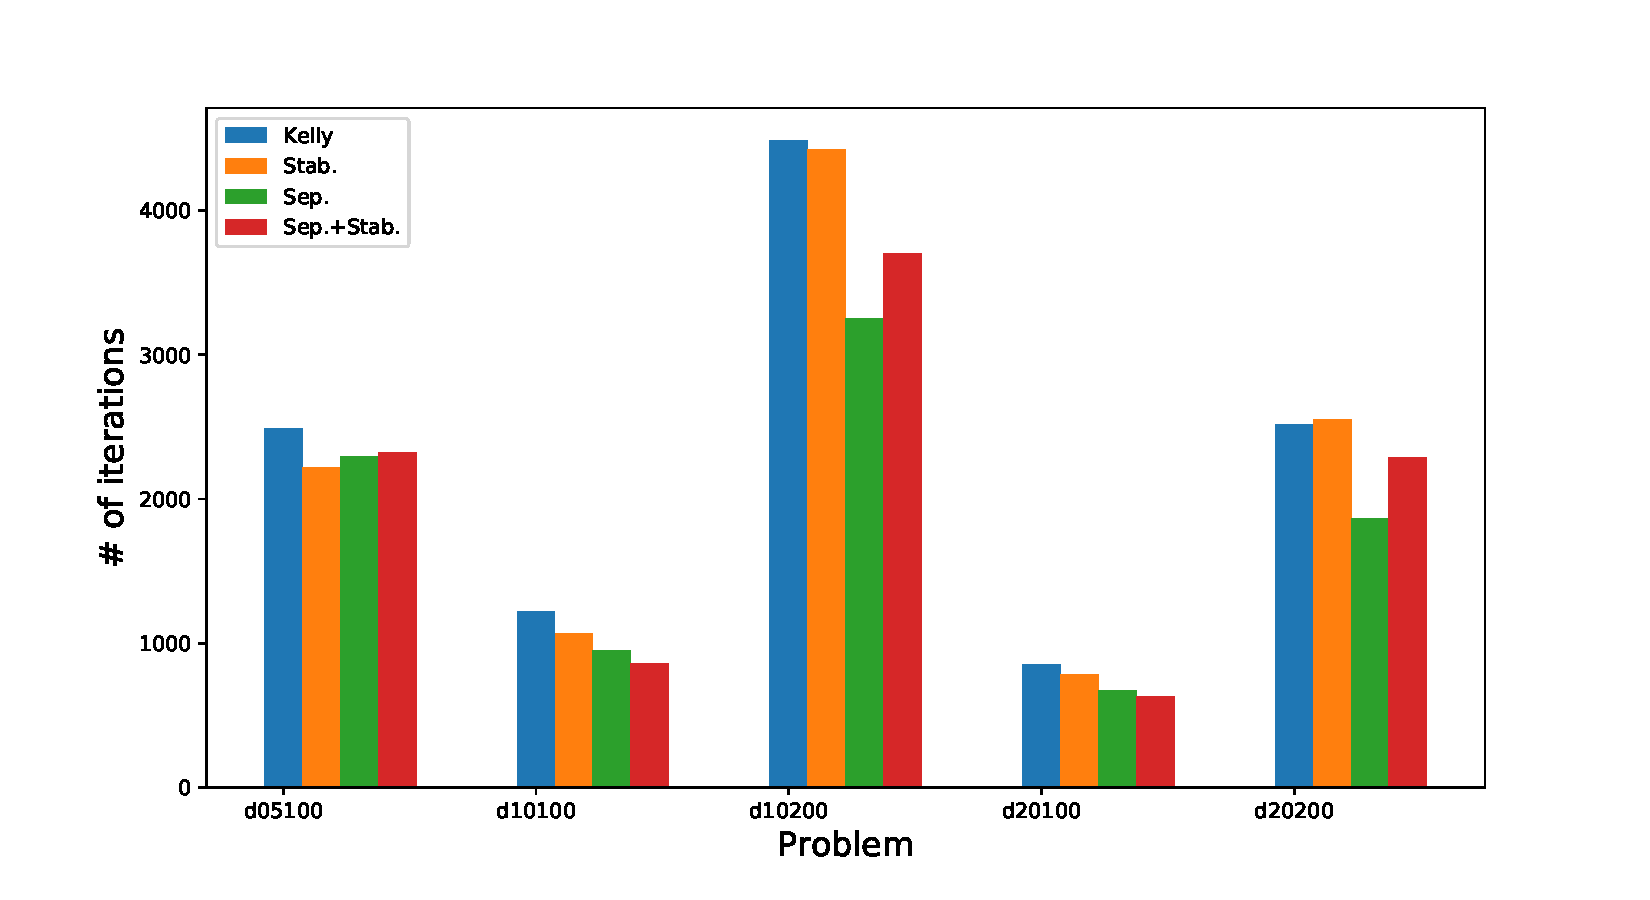
\includegraphics[width=0.8\textwidth]{d}
\caption{ Performance comparison of the algorithms (gap\_d)}
	\end{center}
\end{figure}


\begin{figure}[] 
	\begin{center}
		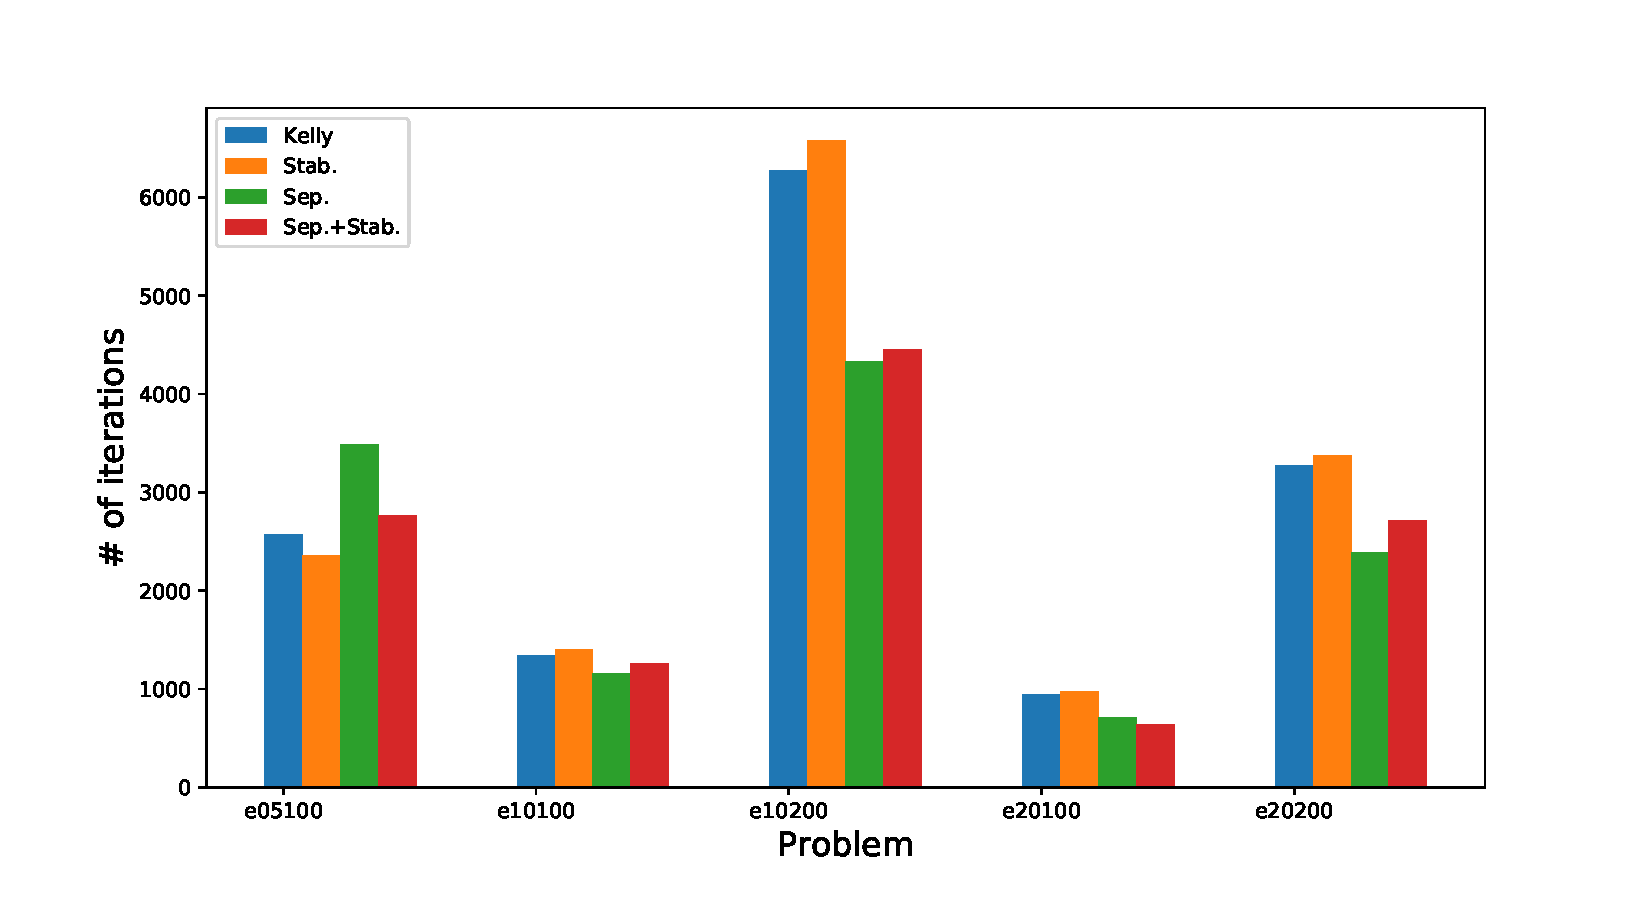
\includegraphics[width=0.8\textwidth]{e}
		\caption{ Performance comparison of the algorithms (gap\_e)}
	\end{center}
\end{figure}
\end{document}